\documentclass[pdftex,12pt,a4paper]{article}

\usepackage[pdftex]{graphicx}
\usepackage{verbatim}
\usepackage{url}

\newcommand{\nesc}{\emph{nesC}}
\newcommand{\code}[1] {{\small{\texttt{#1}}}}

\begin{document}

\begin{titlepage}
\begin{center}

\textsc{\LARGE PUC--Rio}\\[1.5cm]
\textsc{\Large Proposta de Tese de Doutorado}\\[0.5cm]

\newcommand{\HRule}{\rule{\linewidth}{0.5mm}}
\HRule \\[0.4cm]
{ \huge \bfseries Safe and High-level Programming for Embedded Systems}\\[0.4cm]
\HRule \\[1.5cm]

\begin{minipage}{0.4\textwidth}
\begin{flushleft} \large
\emph{Autor:}\\
Francisco Sant'Anna
\end{flushleft}
\end{minipage}
\begin{minipage}{0.4\textwidth}
\begin{flushright} \large
\emph{Orientadores:} \\
Roberto Ierusalimschy \\
Noemi Rodriguez
\end{flushright}
\end{minipage}

\vfill
{\large \today}
\end{center}
\end{titlepage}

\tableofcontents

\section{Introduction}
\label{sec:introduction}

Embedded systems combine hardware, software, and possibly mechanical devices to 
perform a specific dedicated task.
They differ from general-purpose systems, which are designed with flexibility 
in mind and encompass a multitude of applications in a single system.
Examples of embedded systems range from simple MP3 players to complex 
fly-by-wire avionic systems.
Usually they have low tolerance to faults, are constrained in memory and 
processing, and must conform with real-time requirements.~\cite{es.lee}

Embedded systems are essentially reactive as they interact permanently with the 
surrounding environment through input and output devices (e.g. sensors, 
buttons, timers, touch displays, etc.).

% TODO: ref
Software for embedded systems is usually developed in $C$, and the addition of 
a real-time operating system may extend it with preemptive and/or cooperative 
multithreading (\emph{MT})~\cite{wsn.protothreads}.
However, concurrency in $C$ requires a low-level exercise related to the life 
cycle of activities (i.e. creating, starting, and destroying threads), besides 
extra efforts for explicit scheduling (in cooperative \emph{MT}) and manual
synchronization (in preemptive \emph{MT}).
Furthermore, these models lack safety warranties, given that 
cooperative \emph{MT} is susceptible to unbounded execution, while 
preemptive \emph{MT} is subject to race conditions and deadlocks.

An established alternative to $C$ in the field of safety-critical embedded 
systems are the reactive synchronous languages \cite{rp.twelve}.
Two major styles of synchronous languages have evolved:
in the \emph{control}--\emph{imperative} style (e.g. Esterel 
\cite{esterel.design}), programs are structured with control flow primitives, 
such as parallelism, repetition, and preemption;
in the \emph{dataflow}--\emph{declarative} style (e.g. Lustre 
\cite{lustre.ieee91}), programs can be seen as graphs of values, in which a 
change to a value is propagated through its dependencies without explicit 
programming.

\begin{comment}
In the synchronous programming model, concurrent lines of execution advance in 
synchronized steps in reaction to input events from the environment, one at a 
time.
Hence, if a given line of execution is reacting to an event, all other lines of 
execution can only be reacting to the same event (or not executing at all).
The synchronous abstraction makes reasoning about time easier, as concurrent 
activities in a program always share the same external time reference.
\end{comment}

% Thesis Statement

We believe that embedded systems development can benefit from a new programming 
language paradigm that unifies both control and dataflow reactive synchronous 
styles, while preserving typical $C$ features that programmers are familiar 
with, namely shared memory concurrency.

The central idea of our thesis is to pursue the \emph{least common denominator} 
between the two styles, i.e., a programming language with the smallest set of 
primitives that supports both control and dataflow synchronous styles.

In our proposed programming language, by starting from a small synchronous 
control core and extending it with shared memory, we can derive dataflow 
programming without any specific primitives for this purpose.
The synchronous core is very similar to the Esterel programming 
language~\cite{esterel.design}.
On top of it, we introduce controlled side effects, in which variables can be 
shared among multiple lines of execution, and the compiler is responsible for 
detecting race conditions at compile time.

Besides offering high-level reactive programming, a primeval goal in our work 
is to ensure the correctness of programs through safety warranties.
Our proposed semantics enables a compile-time analysis that detects unbounded 
loops and concurrent access to variables.

The static analysis precludes any dynamic support in the language, such as 
memory allocation, a call stack, and dynamic loading.
However, this trade-off seems to be favorable in the context of embedded 
systems, as dynamic features are discouraged due to resource limitations and 
safety requirements.

We have a working implementation of our model as the \emph{C\'eu
programming language}, which is available online%
\footnote{\url{http://www.ceu-lang.org/}}.
C\'eu is targeted at highly constrained embedded platforms, such as Arduino and 
wireless sensor nodes.
\begin{comment}
The current memory footprint of the C\'eu runtime is around 4Kbytes of ROM and 
100bytes of RAM on a 16 bits platform.
\end{comment}

\section{Related work}
\label{sec:related}

In this section, we present a review of some synchronous languages and 
techniques that relate to our research.

\subsection{Event-driven programming}

At the lowest abstract level of the synchronous model, event-driven programming 
is usually employed as a technique in general-purpose languages with no 
specific support for reactivity.
Because a single line of execution and stack are available, programmers need to 
deal with the burden of manual stack management and inversion of 
control.~\cite{sync_async.cooperative}

In the context of embedded systems, the programming language 
\nesc{}~\cite{wsn.nesc} offers event-driven programming for the 
TinyOS~\cite{wsn.tos} operating system.
The concurrency model of \nesc{} is very flexible, supporting the traditional 
serialization among callbacks, and also asynchronous callbacks that interrupt 
others.
To deal with race conditions, \nesc{} supports atomic sections with a similar 
semantics to mutual exclusion in asynchronous languages.

\subsection{Cooperative multithreading}

Cooperative multithreading is an alternative approach to preemptive 
multithreading where the programmer is responsible for scheduling activities in 
the program (known as \emph{coroutines}~\cite{lua.coroutines} in this context).
With this approach, there are no possible race conditions on global variables, 
as the points that transfer control in coroutines are explicit (and, 
supposedly, are never inside critical sections).

Protothreads \cite{wsn.protothreads} offer very lightweight cooperative 
multithreading for embedded systems.
Its stackless implementation reduces memory consumption but precludes support 
for local variables.
Furthermore, Protothreads provide no safety warranties besides being race-free: 
a program can loop indefinitely, and access to globals is unrestricted.

\subsection{Finite state machines}

The use of finite state machines (FSMs) is a classic technique to implement
reactive applications, such as network protocols and graphical user interfaces.
A contemporary work~\cite{wsn.osm}, based on the Statecharts formalism 
\cite{statecharts.visual}, provides a textual FSM language targeting Wireless 
Sensor Networks.

FSMs have some known limitations.
For instance, writing purely sequential flow is tedious, requiring to break 
programs in multiple states with a single transition connecting each of them.  
Another inherent problem of FSMs is the state explosion phenomenon.
To alleviate this problem, some designs support hierarchical FSMs running in 
parallel \cite{wsn.osm}.
However, adopting parallelism precludes the use of shared variables.

%- mostrar a saida de quantos dfa tem cada um dos exemplos
%- ship tem que tirar o async
%- dizer que um programa equivalente teria esse mesmo numero de estados
%e seria impossivel de programar

%- possibly graphical languages (fosters visual) (inherent)

\subsection{Dataflow}

Dataflow programming \cite{lustre.ieee91,lucid,frp.principles} differs from the 
traditional ``Von Neumann'' imperative style, where programs are defined as 
sequences of steps.
With a declarative style, dataflow programs define high-level dependency 
relationships among data.
The language is responsible for scheduling activities that propagate external 
changes into the dependency graph that represents a program.

\begin{comment}
As an example, programs in Lustre~\cite{lustre.ieee91} are composed of 
\emph{nodes} with input edges and an output edge.
Multiple nodes are connected to form a graph that represents a program.
On each clock tick, a node reads its input values and computes its output 
value, which may be connected as input to another node.

The following example illustrates the programming style of Lustre:

{\small
\begin{verbatim}
    node Count (evt, reset: bool)
               returns (count: int);
    let
      count =
        if (true -> reset) then
          0
        else
          if evt then pre(count) + 1
                 else pre(count)
    tel
\end{verbatim}
}

The \code{Count} node represents a flow of \code{int} data that counts the 
number of occurrences of the input \code{evt}.
Whenever the input \code{reset} is true, the node outputs 0; otherwise it 
increments its previous output whenever the input \code{evt} is present.
\end{comment}

Embedded systems are typically characterized by control-intensive applications, 
where programs have to deal with low-level I/O and handle explicit state.
In this context, dataflow programming does not provide proper abstractions, 
being more suitable for data-intensive applications.

\subsection{Esterel}

Our proposed language is strongly influenced by the Esterel language 
\cite{esterel.design}, which also provides an imperative reactive style with a 
similar set of parallel compositions.

The following example illustrates the programming style of Esterel:

{\small
\begin{verbatim}
    1: module ABRO:
    2: input A, B, R;
    3: output O;
    4: loop
    5:   [ await A || await B ];
    6:   emit O
    7: each R
    8: end module
\end{verbatim}
}

The program awaits the input signals \code{A} and \code{B} in parallel (line 
5).
After they both occur, regardless of the order, the program emits the output 
signal \code{O} (line 6) and restarts the process.
If the input signal \code{R} occurs (line 7), the loop also restarts, without 
emitting \code{O}.

In Esterel, the semantics for time is similar to that of digital circuits, 
where an external clock defines discrete steps in which multiple signals can be 
active.

Esterel has no support for shared-memory concurrency, and ``if a variable is 
written in a thread, then it can be neither read nor written in any concurrent 
thread''.~\cite{esterel.primer}

\section{Proposed model}

In our proposed language, multiple lines of execution---known as 
\emph{trails}---continuously react to input events from the environment.
Waiting for an event suspends the running trail until that event occurs.
The environment broadcasts an occurring event to all active trails, which share 
a single global time reference (the event itself).

To illustrate the concurrent reactive nature of the language, the example in 
Figure~\ref{lst:ceu:1} executes three trails in parallel through the \code{par} 
statement.
The program increments a variable every 1 second, which may be reset by an 
external event.
Every time the variable changes, its current value is displayed on screen.

\begin{figure}[t]
\rule{8.5cm}{0.37pt}
{\small
\begin{verbatim}
 1:  input int Restart;     // an external event
 2:  event void changed;    // an internal event
 3:  int v = 0;             // a variable
 4:  par do
 5:     loop do             // 1st trail
 6:        await 1s;
 7:        v = v + 1;
 8:        emit changed;
 9:     end
10:  with
11:     loop do             // 2nd trail
12:        v = await Restart;
13:        emit changed;
14:     end
15:  with
16:     loop do             // 3rd trail
17:        await changed;
18:        _printf("v = %d\n", v);
19:     end
20:  end
\end{verbatim}
}
\caption{ An example.
\label{lst:ceu:1}
}
\end{figure}

Lines 1-3 declare the variables and events used in the program.
The declarations include the type of value the occurring event communicates.
For instance, the external event \code{Restart} carries integer values, while 
the internal event \code{changed} is a notify-only event, holding no values.

The loop in the first trail (lines 5-9) waits for 1 second, increments variable 
\code{v}, and notifies changes through the \code{emit} statement (line 8).
The loop in the second trail (lines 11-14) resets \code{v} to the value of 
every occurrence of the input event \code{Restart} (line 12), and notifies 
these changes (line 13).
The loop in the third trail (lines 16-19) shows the value of \code{v} (line 18) 
whenever the event \code{change} is emitted (line 17).

The execution model is grounded on a precise definition of time as a discrete 
sequence of external input events:
a sequence because only a single input event is handled at a time; discrete 
because a complete reaction always executes in bounded time (to be discussed 
further).

\begin{comment}
The execution model for a program is as follows:

\begin{enumerate}
\setlength{\itemsep}{0pt}
\item The program initiates the ``boot reaction'' in a single trail.
\item Active trails execute until they await or terminate.
      This step is named a \emph{reaction chain}, and always runs in bounded 
      time.
\item If there are no remaining awaiting trails, the program terminates.
      Otherwise, the program goes idle and the environment takes control.
\item On the occurrence of a new external input event, the environment awakes 
      the trails awaiting that event.
      It then goes to step 2.
\end{enumerate}

When multiple trails are active at a time, the order in which they should 
execute is not specified.
The language runtime is allowed to serialize, interleave, or even parallelize 
their execution.

If a new external input event occurs while a reaction chain is running (step 
2), the environment enqueues it to run in the next reaction, because reaction 
chains must run to completion.
\end{comment}

\subsection{Safety warranties}

One of our goals is to provide safe concurrent programming.
Considering the context of embedded systems, it is important that all safety 
warranties are given at compile time.
Currently, we propose two compile time verifications that enforce safety 
restrictions.

The first verification ensures that loops in the language do not run in 
unbounded time making programs unresponsive to handle upcoming input events.
We propose that each possible path in a loop body must contain at least one 
\code{await} or \code{break} statement.
For instance, based on this restriction, the following loops are refused at 
compile time:

{\small
\begin{verbatim}
    // ex. 1:            // ex. 2:
    loop do              loop do
       v = v + 1            if v then
    end                        await A;
                            end     // else does not await
                         end
\end{verbatim}
}
Conversely, the following loops should be accepted:
{\small
\begin{verbatim}
    // ex. 3:            // ex. 4:
    loop do              loop do
       await A;             if v then
    end                        await A;
                            else
                               await B;
                            end
                         end
\end{verbatim}
}

By structural induction on the program AST, it is trivial to infer whether a 
given loop body satisfies that restriction or not.

The second verification ensures that access to shared-memory never occurs 
concurrently in different trails running during the same reaction.

For instance, in the following nondeterministic example, the assignments run 
concurrently:
{\small
\begin{verbatim}
        int v;
        par do
            v = 1;
        with
            v = 2;
        end
\end{verbatim}
}
while in
{\small
\begin{verbatim}
        input void A, B;
        int v;
        par do
            await A;
            v = 1;
        with
            await B;
            v = 2;
        end
\end{verbatim}
}
there is no possible concurrency between the assignments, as $A$ and $B$ are 
external events and, by definition, cannot happen at the same time.

We propose a static analysis at compile time that generates a deterministic 
finite automata representing a program that covers exactly all possible points 
it can reach during runtime.
% TODO: claim

\begin{figure}[t]
\rule{8.5cm}{0.37pt}
{\small
\begin{verbatim}
    input void A;
    int v;
    par do
       loop do
          await A;
          await A;
          v = 1;
       end
    with
       loop do
          await A;
          await A;
          await A;
          v = 2;
       end
    end
\end{verbatim}
}
\caption{ A nondeterministic program.
\label{lst:ceu:det}
}
\end{figure}

\begin{figure}[t]
\centering
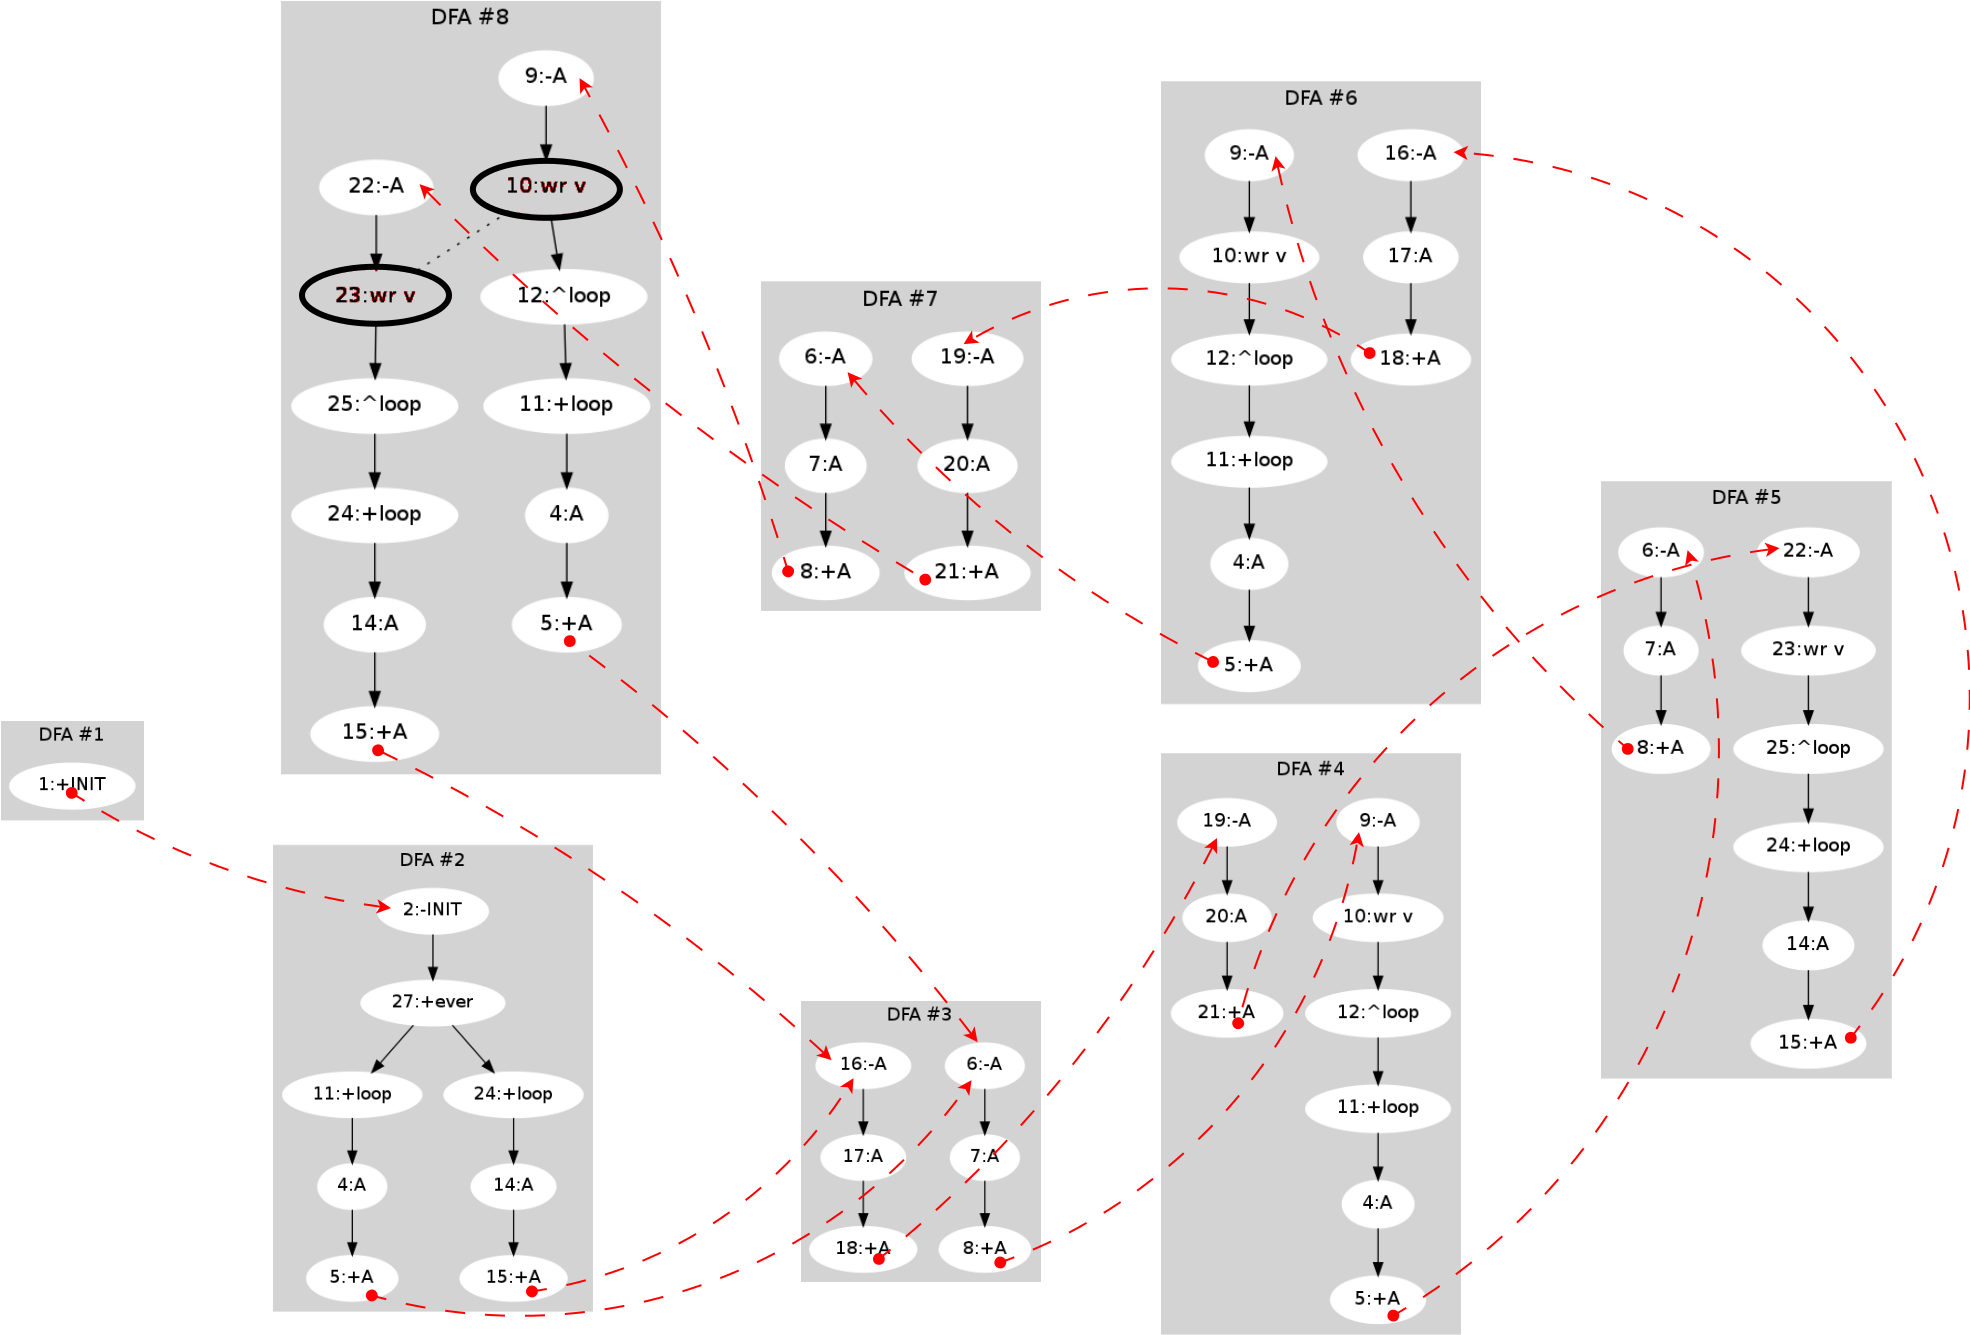
\includegraphics[scale=0.23]{dfa.png}
\caption{ DFA for the nondeterministic example.
\label{fig:dfa}
}
\end{figure}

As an example, the program in Figure~\ref{lst:ceu:det} has the corresponding 
DFA in Figure~\ref{fig:dfa}.
In state \emph{DFA \#8} (after six occurrences of $A$) the variable \code{v} is 
accessed concurrently (note the outlined nodes), qualifying a nondeterministic 
behavior in the program, which is refused at compile time.

\subsection{Internal events \& Dataflow support}
\label{sec:ceu:frp}

Internal events bring dataflow support to the language, allowing that programs 
create dependency relationships among variables.

Suppose in a program we want that any change to variable \code{v1} 
automatically updates \code{v2} to \code{v2=v1+1}, and that any change to 
\code{v2} updates \code{v3} to \code{v3=v2*2}.
The program in Figure~\ref{lst:ceu:frp:1} implements the desired behavior.

% TODO: figura 2 reactions

\begin{figure}[t]
\rule{8.5cm}{0.37pt}
{\small
\begin{verbatim}
 1:  int v1, v2, v3;
 2:  internal void v1_evt, v2_evt, v3_evt;
 3:  par do
 4:     loop do              // 1st trail
 5:        await v1_evt;
 6:        v2 = v1 + 1;
 7:        emit v2_evt;
 8:     end
 9:  with
10:     loop do              // 2nd trail
11:        await v2_evt;
12:        v3 = v2 * 2;
13:        emit v3_evt;
14:     end
15:  with
16:     ...                  // 3rd trail
17:  end
\end{verbatim}
}
\caption{ A dataflow program.
\label{lst:ceu:frp:1}
}
\end{figure}

We start by defining the variables and corresponding internal events to signal 
changes (lines 1-2).
Any change to a variable in the program must be followed by an emit on the 
corresponding event so that dependent variables can react.
Then, we create two trails, one for each dependency relation, to await for 
changes and update the variables.
For instance, the first trail is a \code{loop} (lines 4-8) that waits for 
changes on \code{v1} (line 5), resets \code{v2} to apply the constraint (line 
6), and signals this change (line 7) to make sure that its dependencies are 
also updated.
The behavior for the second trail (lines 10-14), which updates \code{v3} 
whenever \code{v2} changes, is similar.

\subsection{Expected contributions}

The goal of our research is to provide safe and high-level programming for 
embedded systems.

Regarding high-level programming, the first contribution is the unification of 
control and dataflow reactivity in a single language.
Both styles provide powerful abstractions for programming embedded systems, but 
we are not aware of a single language that addresses both styles.
We propose a control core similar to the Esterel programming language and 
include shared state to also support the dataflow style.
Another contribution is first-class support for \emph{wall-clock} time (i.e.  
time from the real world, measured in hours, minutes, etc.), which is probably 
the most common input in embedded systems, as found in typical patterns like 
sensor samplings and watchdogs.

Regarding safety, we propose a deterministic execution model in which only a 
single input event can occur at a time.
To contrast with Esterel, in which time is defined as a sequence of \emph{tick} 
pulses in which multiple events can coexist, our modification enables the 
proposed static temporal analysis that detects concurrent access to shared 
state.
We also propose a compile-time verification to ensure that loops always run in 
bounded time.

Finally, we show the viability of our model in the context of embedded systems 
with an implementation targeting highly constrained platforms.

\section{Work plan}

Our current activities can be split in three different fronts:

\begin{description}

\item[Language design:]
The overall language design is satisfactory and we do not expect to add new 
features or dramatically change the current semantics.
The next step is to work on a precise description, possibly with the formal 
operational semantics of the language.

\item[Target platforms:]
To test the viability of the language in the context of embedded systems, we 
have been evaluating two embedded platforms.
The activity in this area constitutes the integration of the language with the 
environment, i.e., the definition of input \& output events, and the mechanisms 
for acquisition (e.g. polling vs ISRs).

A challenge is to keep the language runtime with a low memory overhead to 
permit the development of complex applications.
For the platforms we have been working, the runtime is around 10\% of the total 
available memory.
We expect to port the runtime to even more constrained microcontrollers, such 
as the \emph{PIC-16} family.

\item[Application scenarios:]
In order to evaluate our research goals of providing safe and high-level 
programming for embedded systems, we intend to apply our language to different
application scenarios.
Currently, we have been working with wireless sensor networks (WSNs), 
developing a library of distributed algorithms to be used in networked 
applications.

We will use quantitative and qualitative metrics in our evaluation.
As an example, an existing work \cite{wsn.comparison} measures the performance 
of different programming languages regarding memory usage, battery consumption, 
and responsiveness specifically for WSNs.
These aspects are of extreme importance, given the severe hardware constraints 
in this context.

\subsection{Schedule}

\end{description}

\begin{table}[h]
\begin{center}
\begin{tabular}{ | l | c | c | c | c | c | }
\hline
 & jul-sep & oct-dec & jan-mar & apr-jun & jul-sep \\ \hline
New platforms          & x & x & x &   &   \\ \hline
Language evaluation    & x & x & x & x &   \\ \hline
    - WSNs             & x & x &   &   &   \\ \hline
    - New scenarios    &   & x & x &   &   \\ \hline
Language formalization &   &   &   & x & x \\ \hline
Thesis writing         &   &   &   & x & x \\ \hline
\end{tabular}
\end{center}
\end{table}

\begin{comment}

\begin{description}
\item[Unification of Control and Dataflow synchronous programming]
\item[Ciclos]
\item[Time]
\item[Asynchronous]
\end{description}

\section{Background}

Consider the hypothetical concurrent example, as follows:

{\small
\begin{verbatim}
    input A, B;
    int v;
    [ await A;
      v = 1;
    ||
      await B
      v = 2;
    ];
\end{verbatim}
}

Hence, in the previous chunk, both signals \code{A} and \code{B} in parallel 
threads can be active at a time, making the assignment to \code{v} 
nondeterministic.

- useful
    - control
        - hierarchical state machines, protocols, device drivers
    - dataflow
        - streams, DSP, filters
    - BOTH are rigorous models

    - shared memory
        - general purpose
        - matches underlying architecture
        - not rigorous

- both styles are useful
- no languages does this
    - what are the least common?
        - control is lower level

- shared memory is popular
    - better performance / matches underlying architecture (important for ES)
    - avoid use of other synchronizations
    - take advantage of synch semantics

- what we loose
    - dynamic
    - there are dyn dataflow / FRP
    - there are dyn shared-memory / threads

The main objective of our thesis is to address

    how to support control and dataflow reactive programming
    what are the least common among them?

    how to support shared memory

-, no such language exists
- how to support shared memory safely and seamlessly, without requiring the 
  programmer efforts
- turns out that Esterel + SE => dataflow
- disciplined synchronous execution enables

- side contributions
    - time
    - ciclos
    - compositions
    - asyncs

=============
Coroutines are similar to \CEU{} trails, as they both offer multiple sequential 
lines of execution to handle concurrent activities.
However, \CEU{}'s \code{par/and} and \code{par/or} composition statements offer 
a powerful abstraction to avoid manual bookkeeping of activities, such as 
creating, starting, rejoining, and destroying them.
Also, the semantics for rejoins in parallel compositions is fundamental for the 
temporal analysis of \CEU{}, which cannot be done effectively with coroutines.

or at least requires a static analysis such as that of \CEU{}.

\CEU{} borrows some ideas from a FRP implementation \cite{frtime.embedding}, 
such as a push-driven evaluation and glitch prevention.
Dataflow in \CEU{} is limited to static relationships, and the way dataflow 
programs are expressed is less abstract than in FRP.

Regarding features that are orthogonal to the distinction regarding events, 
\CEU{} supports ``wall-clock'' time and simulation from asynchronous blocks, 
while Esterel provides a \code{suspend} statement that cannot be easily 
implemented on top of the existing primitives (and which we are considering to 
incorporate into \CEU).

% TODO
Esterel also supports output events, which are not available in \CEU{}.
Also, \CEU{} has no support for output events, and relies on $C$ calls to 
interface with the environment for output.
If multiple processes in \CEU{} needed to communicate, the adoption of output; 
however, in the context of embedded systems, only a single process executes at 
a time.
\end{comment}

    \nocite{ds.andrews}
    \nocite{sync.colors}
    \nocite{sync_async.duality}
    \nocite{sync_async.threadsstop}
    \nocite{sync_async.whynotthreads}
    \nocite{sync_async.whynotevents}
    \nocite{async.csp}
    \nocite{async.monitors}
    \nocite{rp.hypothesis}
    \nocite{frp.fran}
    \nocite{frtime.adapting}
    \nocite{arduino.occam}
    \nocite{wsn.survey}
    \nocite{wsn.contiki}
    \nocite{wsn.sol}
    \nocite{wsn.mantisos}
    \nocite{wsn.flask}

\bibliographystyle{acm}
\bibliography{other}

\end{document}
